\documentclass[1p]{elsarticle_modified}
%\bibliographystyle{elsarticle-num}

%\usepackage[colorlinks]{hyperref}
%\usepackage{abbrmath_seonhwa} %\Abb, \Ascr, \Acal ,\Abf, \Afrak
\usepackage{amsfonts}
\usepackage{amssymb}
\usepackage{amsmath}
\usepackage{amsthm}
\usepackage{scalefnt}
\usepackage{amsbsy}
\usepackage{kotex}
\usepackage{caption}
\usepackage{subfig}
\usepackage{color}
\usepackage{graphicx}
\usepackage{xcolor} %% white, black, red, green, blue, cyan, magenta, yellow
\usepackage{float}
\usepackage{setspace}
\usepackage{hyperref}

\usepackage{tikz}
\usetikzlibrary{arrows}

\usepackage{multirow}
\usepackage{array} % fixed length table
\usepackage{hhline}

%%%%%%%%%%%%%%%%%%%%%
\makeatletter
\renewcommand*\env@matrix[1][\arraystretch]{%
	\edef\arraystretch{#1}%
	\hskip -\arraycolsep
	\let\@ifnextchar\new@ifnextchar
	\array{*\c@MaxMatrixCols c}}
\makeatother %https://tex.stackexchange.com/questions/14071/how-can-i-increase-the-line-spacing-in-a-matrix
%%%%%%%%%%%%%%%

\usepackage[normalem]{ulem}

\newcommand{\msout}[1]{\ifmmode\text{\sout{\ensuremath{#1}}}\else\sout{#1}\fi}
%SOURCE: \msout is \stkout macro in https://tex.stackexchange.com/questions/20609/strikeout-in-math-mode

\newcommand{\cancel}[1]{
	\ifmmode
	{\color{red}\msout{#1}}
	\else
	{\color{red}\sout{#1}}
	\fi
}

\newcommand{\add}[1]{
	{\color{blue}\uwave{#1}}
}

\newcommand{\replace}[2]{
	\ifmmode
	{\color{red}\msout{#1}}{\color{blue}\uwave{#2}}
	\else
	{\color{red}\sout{#1}}{\color{blue}\uwave{#2}}
	\fi
}

\newcommand{\Sol}{\mathcal{S}} %segment
\newcommand{\D}{D} %diagram
\newcommand{\A}{\mathcal{A}} %arc


%%%%%%%%%%%%%%%%%%%%%%%%%%%%%5 test

\def\sl{\operatorname{\textup{SL}}(2,\Cbb)}
\def\psl{\operatorname{\textup{PSL}}(2,\Cbb)}
\def\quan{\mkern 1mu \triangleright \mkern 1mu}

\theoremstyle{definition}
\newtheorem{thm}{Theorem}[section]
\newtheorem{prop}[thm]{Proposition}
\newtheorem{lem}[thm]{Lemma}
\newtheorem{ques}[thm]{Question}
\newtheorem{cor}[thm]{Corollary}
\newtheorem{defn}[thm]{Definition}
\newtheorem{exam}[thm]{Example}
\newtheorem{rmk}[thm]{Remark}
\newtheorem{alg}[thm]{Algorithm}

\newcommand{\I}{\sqrt{-1}}
\begin{document}

%\begin{frontmatter}
%
%\title{Boundary parabolic representations of knots up to 8 crossings}
%
%%% Group authors per affiliation:
%\author{Yunhi Cho} 
%\address{Department of Mathematics, University of Seoul, Seoul, Korea}
%\ead{yhcho@uos.ac.kr}
%
%
%\author{Seonhwa Kim} %\fnref{s_kim}}
%\address{Center for Geometry and Physics, Institute for Basic Science, Pohang, 37673, Korea}
%\ead{ryeona17@ibs.re.kr}
%
%\author{Hyuk Kim}
%\address{Department of Mathematical Sciences, Seoul National University, Seoul 08826, Korea}
%\ead{hyukkim@snu.ac.kr}
%
%\author{Seokbeom Yoon}
%\address{Department of Mathematical Sciences, Seoul National University, Seoul, 08826,  Korea}
%\ead{sbyoon15@snu.ac.kr}
%
%\begin{abstract}
%We find all boundary parabolic representation of knots up to 8 crossings.
%
%\end{abstract}
%\begin{keyword}
%    \MSC[2010] 57M25 
%\end{keyword}
%
%\end{frontmatter}

%\linenumbers
%\tableofcontents
%
\newcommand\colored[1]{\textcolor{white}{\rule[-0.35ex]{0.8em}{1.4ex}}\kern-0.8em\color{red} #1}%
%\newcommand\colored[1]{\textcolor{white}{ #1}\kern-2.17ex	\textcolor{white}{ #1}\kern-1.81ex	\textcolor{white}{ #1}\kern-2.15ex\color{red}#1	}

{\Large $\underline{11n_{120}~(K11n_{120})}$}

\setlength{\tabcolsep}{10pt}
\renewcommand{\arraystretch}{1.6}
\vspace{1cm}\begin{tabular}{m{100pt}>{\centering\arraybackslash}m{274pt}}
\multirow{5}{120pt}{
	\centering
	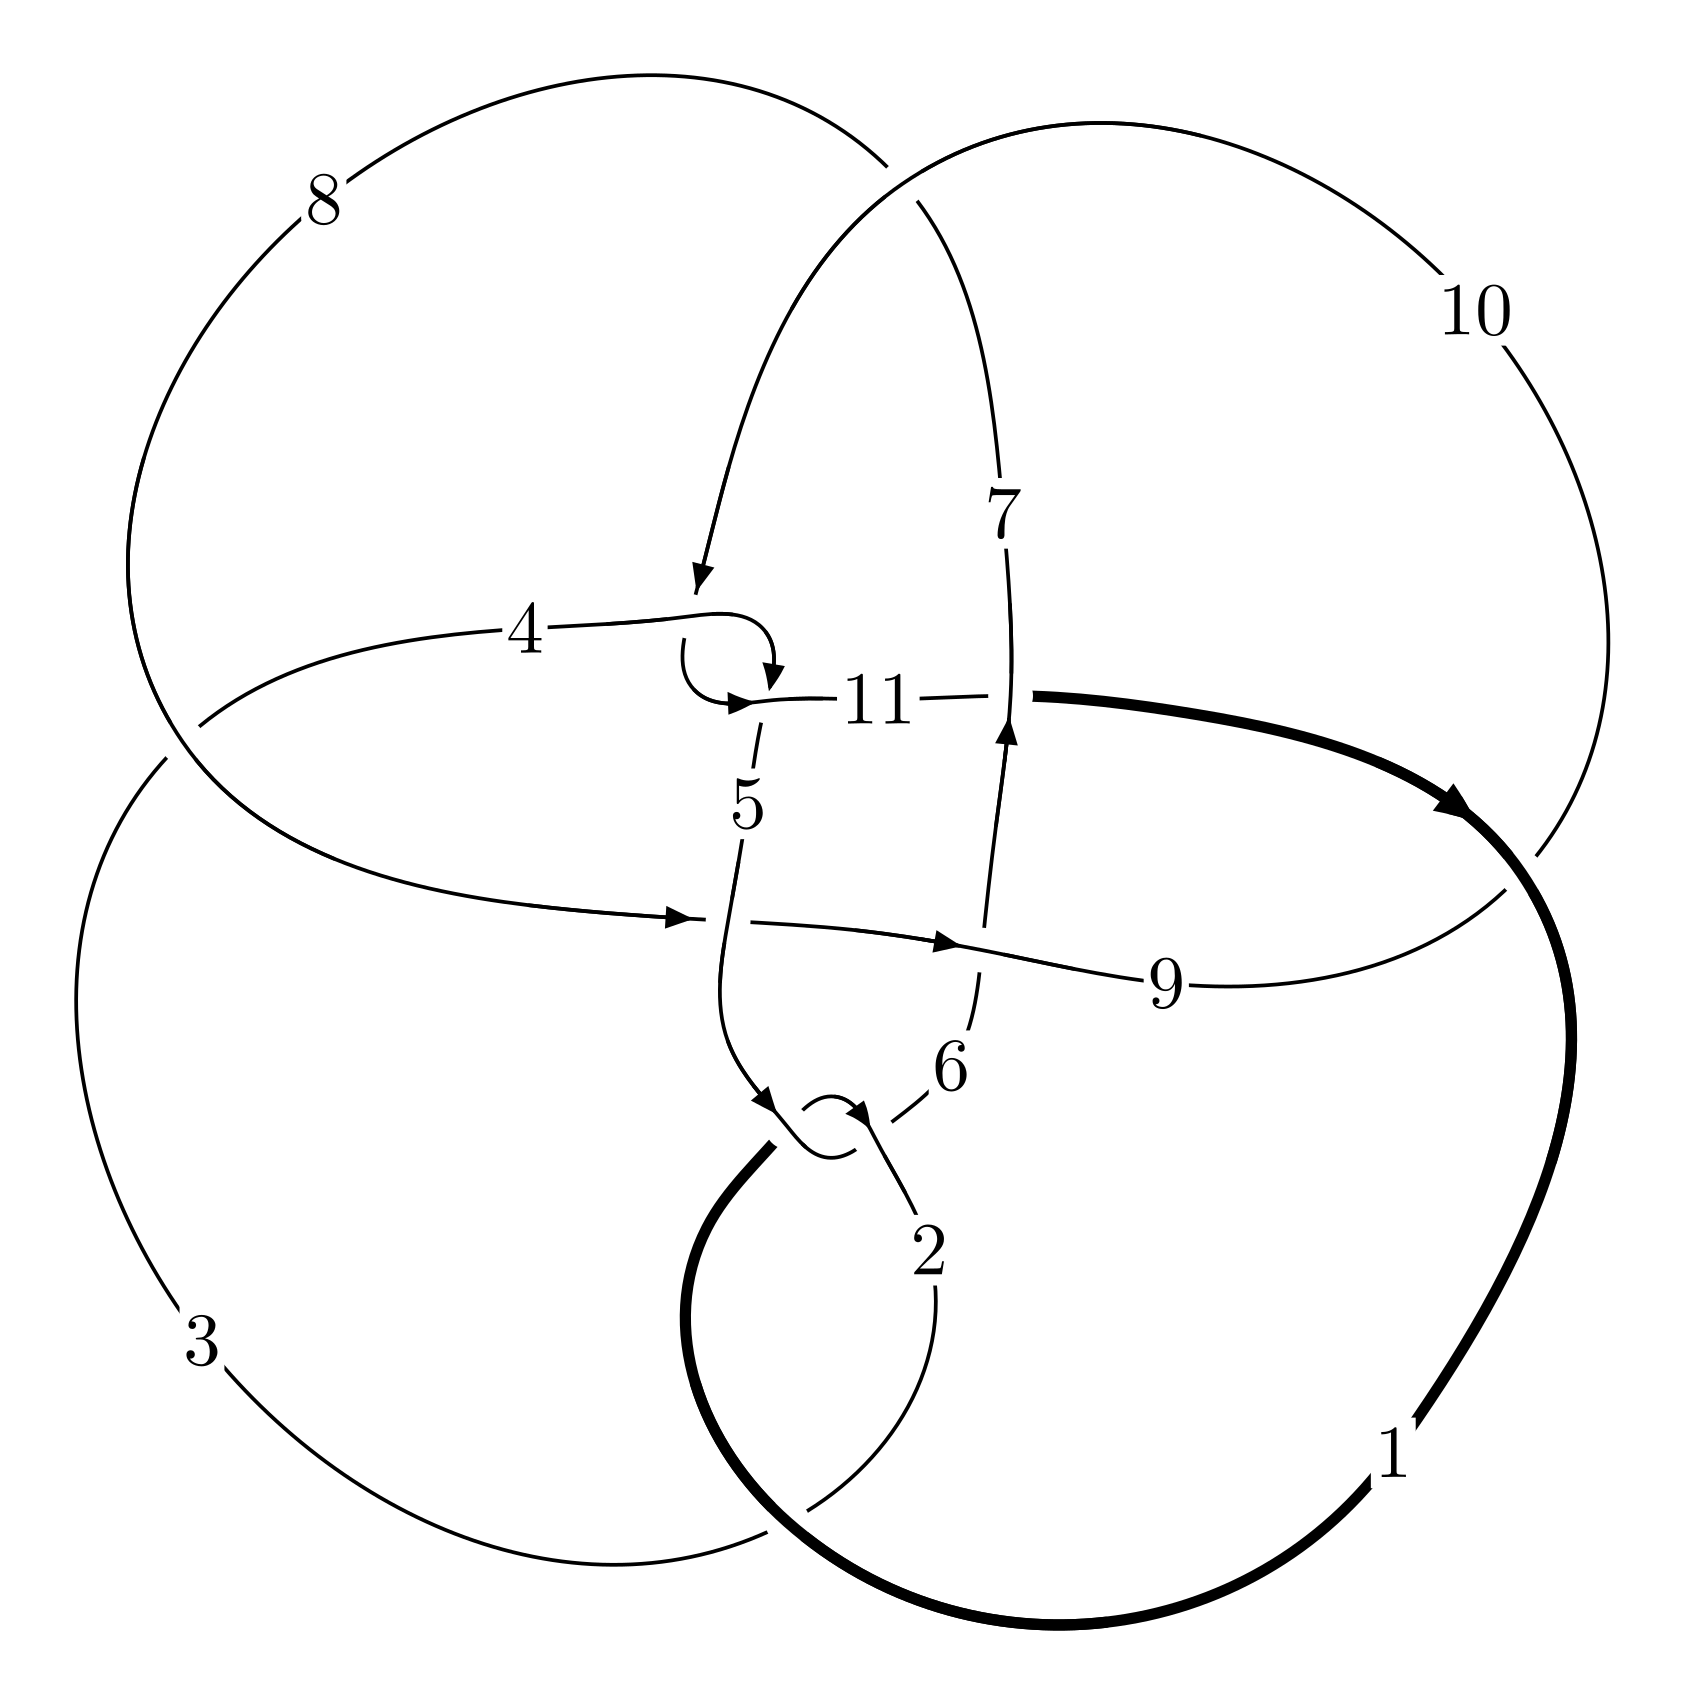
\includegraphics[width=112pt]{../../../GIT/diagram.site/Diagrams/png/736_11n_120.png}\\
\ \ \ A knot diagram\footnotemark}&
\allowdisplaybreaks
\textbf{Linearized knot diagam} \\
\cline{2-2}
 &
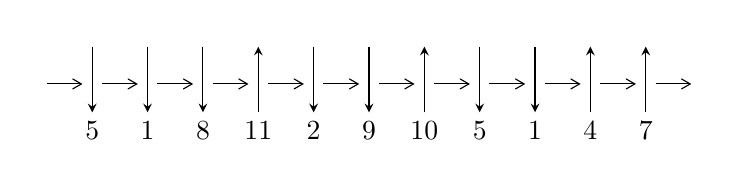
\begin{tikzpicture}[x=20pt, y=17pt]
	% nodes
	\node (C0) at (0, 0) {};
	\node (C1) at (1, 0) {};
	\node (C1U) at (1, +1) {};
	\node (C1D) at (1, -1) {5};

	\node (C2) at (2, 0) {};
	\node (C2U) at (2, +1) {};
	\node (C2D) at (2, -1) {1};

	\node (C3) at (3, 0) {};
	\node (C3U) at (3, +1) {};
	\node (C3D) at (3, -1) {8};

	\node (C4) at (4, 0) {};
	\node (C4U) at (4, +1) {};
	\node (C4D) at (4, -1) {11};

	\node (C5) at (5, 0) {};
	\node (C5U) at (5, +1) {};
	\node (C5D) at (5, -1) {2};

	\node (C6) at (6, 0) {};
	\node (C6U) at (6, +1) {};
	\node (C6D) at (6, -1) {9};

	\node (C7) at (7, 0) {};
	\node (C7U) at (7, +1) {};
	\node (C7D) at (7, -1) {10};

	\node (C8) at (8, 0) {};
	\node (C8U) at (8, +1) {};
	\node (C8D) at (8, -1) {5};

	\node (C9) at (9, 0) {};
	\node (C9U) at (9, +1) {};
	\node (C9D) at (9, -1) {1};

	\node (C10) at (10, 0) {};
	\node (C10U) at (10, +1) {};
	\node (C10D) at (10, -1) {4};

	\node (C11) at (11, 0) {};
	\node (C11U) at (11, +1) {};
	\node (C11D) at (11, -1) {7};
	\node (C12) at (12, 0) {};

	% arrows
	\draw[->,>={angle 60}]
	(C0) edge (C1) (C1) edge (C2) (C2) edge (C3) (C3) edge (C4) (C4) edge (C5) (C5) edge (C6) (C6) edge (C7) (C7) edge (C8) (C8) edge (C9) (C9) edge (C10) (C10) edge (C11) (C11) edge (C12) ;	\draw[->,>=stealth]
	(C1U) edge (C1D) (C2U) edge (C2D) (C3U) edge (C3D) (C4D) edge (C4U) (C5U) edge (C5D) (C6U) edge (C6D) (C7D) edge (C7U) (C8U) edge (C8D) (C9U) edge (C9D) (C10D) edge (C10U) (C11D) edge (C11U) ;
	\end{tikzpicture} \\
\hhline{~~} \\& 
\textbf{Solving Sequence} \\ \cline{2-2} 
 &
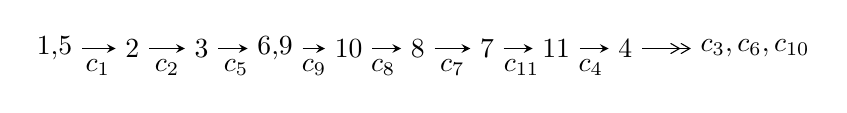
\begin{tikzpicture}[x=25pt, y=7pt]
	% node
	\node (A0) at (-1/8, 0) {1,5};
	\node (A1) at (1, 0) {2};
	\node (A2) at (2, 0) {3};
	\node (A3) at (49/16, 0) {6,9};
	\node (A4) at (33/8, 0) {10};
	\node (A5) at (41/8, 0) {8};
	\node (A6) at (49/8, 0) {7};
	\node (A7) at (57/8, 0) {11};
	\node (A8) at (65/8, 0) {4};
	\node (C1) at (1/2, -1) {$c_{1}$};
	\node (C2) at (3/2, -1) {$c_{2}$};
	\node (C3) at (5/2, -1) {$c_{5}$};
	\node (C4) at (29/8, -1) {$c_{9}$};
	\node (C5) at (37/8, -1) {$c_{8}$};
	\node (C6) at (45/8, -1) {$c_{7}$};
	\node (C7) at (53/8, -1) {$c_{11}$};
	\node (C8) at (61/8, -1) {$c_{4}$};
	\node (A9) at (10, 0) {$c_{3},c_{6},c_{10}$};

	% edge
	\draw[->,>=stealth]	
	(A0) edge (A1) (A1) edge (A2) (A2) edge (A3) (A3) edge (A4) (A4) edge (A5) (A5) edge (A6) (A6) edge (A7) (A7) edge (A8) ;
	\draw[->>,>={angle 60}]	
	(A8) edge (A9);
\end{tikzpicture} \\ 

\end{tabular} \\

\footnotetext{
The image of knot diagram is generated by the software ``\textbf{Draw programme}" developed by Andrew Bartholomew(\url{http://www.layer8.co.uk/maths/draw/index.htm\#Running-draw}), where we modified some parts for our purpose(\url{https://github.com/CATsTAILs/LinksPainter}).
}\phantom \\ \newline 
\centering \textbf{Ideals for irreducible components\footnotemark of $X_{\text{par}}$} 
 
\begin{align*}
I^u_{1}&=\langle 
2.10700\times10^{42} u^{32}-8.32114\times10^{42} u^{31}+\cdots+1.04181\times10^{43} b+3.11913\times10^{43},\\
\phantom{I^u_{1}}&\phantom{= \langle  }-3.50718\times10^{43} u^{32}+1.44547\times10^{44} u^{31}+\cdots+1.04181\times10^{43} a-2.21436\times10^{44},\\
\phantom{I^u_{1}}&\phantom{= \langle  }u^{33}-4 u^{32}+\cdots+20 u+1\rangle \\
I^u_{2}&=\langle 
- u^7- u^6+4 u^5+5 u^4-2 u^3-4 u^2+b+u+1,\;u^9+u^8-5 u^7-6 u^6+6 u^5+9 u^4-4 u^3-6 u^2+a+u+2,\\
\phantom{I^u_{2}}&\phantom{= \langle  }u^{10}+u^9-5 u^8-6 u^7+6 u^6+9 u^5-4 u^4-6 u^3+2 u^2+2 u-1\rangle \\
\\
\end{align*}
\raggedright * 2 irreducible components of $\dim_{\mathbb{C}}=0$, with total 43 representations.\\
\footnotetext{All coefficients of polynomials are rational numbers. But the coefficients are sometimes approximated in decimal forms when there is not enough margin.}
\newpage
\renewcommand{\arraystretch}{1}
\centering \section*{I. $I^u_{1}= \langle 2.11\times10^{42} u^{32}-8.32\times10^{42} u^{31}+\cdots+1.04\times10^{43} b+3.12\times10^{43},\;-3.51\times10^{43} u^{32}+1.45\times10^{44} u^{31}+\cdots+1.04\times10^{43} a-2.21\times10^{44},\;u^{33}-4 u^{32}+\cdots+20 u+1 \rangle$}
\flushleft \textbf{(i) Arc colorings}\\
\begin{tabular}{m{7pt} m{180pt} m{7pt} m{180pt} }
\flushright $a_{1}=$&$\begin{pmatrix}1\\0\end{pmatrix}$ \\
\flushright $a_{5}=$&$\begin{pmatrix}0\\u\end{pmatrix}$ \\
\flushright $a_{2}=$&$\begin{pmatrix}1\\u^2\end{pmatrix}$ \\
\flushright $a_{3}=$&$\begin{pmatrix}- u^2+1\\u^2\end{pmatrix}$ \\
\flushright $a_{6}=$&$\begin{pmatrix}- u\\- u^3+u\end{pmatrix}$ \\
\flushright $a_{9}=$&$\begin{pmatrix}3.36643 u^{32}-13.8746 u^{31}+\cdots+359.454 u+21.2550\\-0.202245 u^{32}+0.798722 u^{31}+\cdots-30.1211 u-2.99396\end{pmatrix}$ \\
\flushright $a_{10}=$&$\begin{pmatrix}3.56868 u^{32}-14.6734 u^{31}+\cdots+389.575 u+24.2489\\-0.202245 u^{32}+0.798722 u^{31}+\cdots-30.1211 u-2.99396\end{pmatrix}$ \\
\flushright $a_{8}=$&$\begin{pmatrix}3.36643 u^{32}-13.8746 u^{31}+\cdots+359.454 u+21.2550\\-0.242116 u^{32}+0.964369 u^{31}+\cdots-34.9325 u-3.40285\end{pmatrix}$ \\
\flushright $a_{7}=$&$\begin{pmatrix}-2.39153 u^{32}+9.65565 u^{31}+\cdots-322.155 u-32.6535\\-0.333028 u^{32}+1.39186 u^{31}+\cdots-27.7757 u-1.13662\end{pmatrix}$ \\
\flushright $a_{11}=$&$\begin{pmatrix}-0.0378953 u^{32}-0.0228553 u^{31}+\cdots-72.9307 u-16.7529\\-0.414218 u^{32}+1.71120 u^{31}+\cdots-42.6953 u-2.83658\end{pmatrix}$ \\
\flushright $a_{4}=$&$\begin{pmatrix}-1.41343 u^{32}+6.01740 u^{31}+\cdots-83.5671 u+7.88298\\0.510036 u^{32}-2.09654 u^{31}+\cdots+58.5090 u+4.26540\end{pmatrix}$\\ \flushright $a_{4}=$&$\begin{pmatrix}-1.41343 u^{32}+6.01740 u^{31}+\cdots-83.5671 u+7.88298\\0.510036 u^{32}-2.09654 u^{31}+\cdots+58.5090 u+4.26540\end{pmatrix}$\\&\end{tabular}
\flushleft \textbf{(ii) Obstruction class $= -1$}\\~\\
\flushleft \textbf{(iii) Cusp Shapes $= 1.43631 u^{32}-5.67419 u^{31}+\cdots+211.371 u+17.0575$}\\~\\
\newpage\renewcommand{\arraystretch}{1}
\flushleft \textbf{(iv) u-Polynomials at the component}\newline \\
\begin{tabular}{m{50pt}|m{274pt}}
Crossings & \hspace{64pt}u-Polynomials at each crossing \\
\hline $$\begin{aligned}c_{1},c_{5}\end{aligned}$$&$\begin{aligned}
&u^{33}+4 u^{32}+\cdots+20 u-1
\end{aligned}$\\
\hline $$\begin{aligned}c_{2}\end{aligned}$$&$\begin{aligned}
&u^{33}+48 u^{32}+\cdots+88 u+1
\end{aligned}$\\
\hline $$\begin{aligned}c_{3}\end{aligned}$$&$\begin{aligned}
&u^{33}- u^{32}+\cdots+864 u-691
\end{aligned}$\\
\hline $$\begin{aligned}c_{4},c_{10}\end{aligned}$$&$\begin{aligned}
&u^{33}-11 u^{31}+\cdots- u-1
\end{aligned}$\\
\hline $$\begin{aligned}c_{6}\end{aligned}$$&$\begin{aligned}
&u^{33}+6 u^{32}+\cdots-2315 u+1751
\end{aligned}$\\
\hline $$\begin{aligned}c_{7}\end{aligned}$$&$\begin{aligned}
&u^{33}+10 u^{32}+\cdots+108 u+11
\end{aligned}$\\
\hline $$\begin{aligned}c_{8}\end{aligned}$$&$\begin{aligned}
&u^{33}-32 u^{31}+\cdots+138 u-193
\end{aligned}$\\
\hline $$\begin{aligned}c_{9}\end{aligned}$$&$\begin{aligned}
&u^{33}-8 u^{32}+\cdots+8781 u-1799
\end{aligned}$\\
\hline $$\begin{aligned}c_{11}\end{aligned}$$&$\begin{aligned}
&u^{33}-2 u^{32}+\cdots+5 u+1
\end{aligned}$\\
\hline
\end{tabular}\\~\\
\newpage\renewcommand{\arraystretch}{1}
\flushleft \textbf{(v) Riley Polynomials at the component}\newline \\
\begin{tabular}{m{50pt}|m{274pt}}
Crossings & \hspace{64pt}Riley Polynomials at each crossing \\
\hline $$\begin{aligned}c_{1},c_{5}\end{aligned}$$&$\begin{aligned}
&y^{33}-48 y^{32}+\cdots+88 y-1
\end{aligned}$\\
\hline $$\begin{aligned}c_{2}\end{aligned}$$&$\begin{aligned}
&y^{33}-124 y^{32}+\cdots-3924 y-1
\end{aligned}$\\
\hline $$\begin{aligned}c_{3}\end{aligned}$$&$\begin{aligned}
&y^{33}-21 y^{32}+\cdots+2800148 y-477481
\end{aligned}$\\
\hline $$\begin{aligned}c_{4},c_{10}\end{aligned}$$&$\begin{aligned}
&y^{33}-22 y^{32}+\cdots+11 y-1
\end{aligned}$\\
\hline $$\begin{aligned}c_{6}\end{aligned}$$&$\begin{aligned}
&y^{33}-58 y^{32}+\cdots+8486511 y-3066001
\end{aligned}$\\
\hline $$\begin{aligned}c_{7}\end{aligned}$$&$\begin{aligned}
&y^{33}+2 y^{32}+\cdots+48 y-121
\end{aligned}$\\
\hline $$\begin{aligned}c_{8}\end{aligned}$$&$\begin{aligned}
&y^{33}-64 y^{32}+\cdots-45418 y-37249
\end{aligned}$\\
\hline $$\begin{aligned}c_{9}\end{aligned}$$&$\begin{aligned}
&y^{33}-36 y^{32}+\cdots+44853489 y-3236401
\end{aligned}$\\
\hline $$\begin{aligned}c_{11}\end{aligned}$$&$\begin{aligned}
&y^{33}+2 y^{32}+\cdots-17 y-1
\end{aligned}$\\
\hline
\end{tabular}\\~\\
\newpage\flushleft \textbf{(vi) Complex Volumes and Cusp Shapes}
$$\begin{array}{c|c|c}  
\text{Solutions to }I^u_{1}& \I (\text{vol} + \sqrt{-1}CS) & \text{Cusp shape}\\
 \hline 
\begin{aligned}
u &= -0.403017 + 0.814677 I \\
a &= \phantom{-}0.107700 - 0.226447 I \\
b &= -0.856763 + 0.231979 I\end{aligned}
 & \phantom{-}2.50185 - 1.42660 I & -0.894808 - 0.237180 I \\ \hline\begin{aligned}
u &= -0.403017 - 0.814677 I \\
a &= \phantom{-}0.107700 + 0.226447 I \\
b &= -0.856763 - 0.231979 I\end{aligned}
 & \phantom{-}2.50185 + 1.42660 I & -0.894808 + 0.237180 I \\ \hline\begin{aligned}
u &= \phantom{-}1.032610 + 0.451125 I \\
a &= -0.534105 + 0.421030 I \\
b &= -0.605715 + 0.947070 I\end{aligned}
 & \phantom{-}0.20621 + 3.24394 I & -3.32595 - 5.32169 I \\ \hline\begin{aligned}
u &= \phantom{-}1.032610 - 0.451125 I \\
a &= -0.534105 - 0.421030 I \\
b &= -0.605715 - 0.947070 I\end{aligned}
 & \phantom{-}0.20621 - 3.24394 I & -3.32595 + 5.32169 I \\ \hline\begin{aligned}
u &= -0.617495 + 0.594331 I \\
a &= \phantom{-}0.228591 + 0.499559 I \\
b &= \phantom{-}0.686667 + 0.747422 I\end{aligned}
 & -0.659531 - 0.792248 I & -4.14798 - 2.75904 I \\ \hline\begin{aligned}
u &= -0.617495 - 0.594331 I \\
a &= \phantom{-}0.228591 - 0.499559 I \\
b &= \phantom{-}0.686667 - 0.747422 I\end{aligned}
 & -0.659531 + 0.792248 I & -4.14798 + 2.75904 I \\ \hline\begin{aligned}
u &= -0.709464 + 0.375757 I \\
a &= -0.54330 - 1.82882 I \\
b &= -1.28499 + 0.81921 I\end{aligned}
 & \phantom{-}1.69477 - 3.95490 I & -4.65099 + 5.53433 I \\ \hline\begin{aligned}
u &= -0.709464 - 0.375757 I \\
a &= -0.54330 + 1.82882 I \\
b &= -1.28499 - 0.81921 I\end{aligned}
 & \phantom{-}1.69477 + 3.95490 I & -4.65099 - 5.53433 I \\ \hline\begin{aligned}
u &= \phantom{-}0.788903 + 0.039022 I \\
a &= -1.048110 - 0.208486 I \\
b &= -0.390987 - 0.219065 I\end{aligned}
 & -1.46450 - 0.11042 I & -7.61890 - 0.69071 I \\ \hline\begin{aligned}
u &= \phantom{-}0.788903 - 0.039022 I \\
a &= -1.048110 + 0.208486 I \\
b &= -0.390987 + 0.219065 I\end{aligned}
 & -1.46450 + 0.11042 I & -7.61890 + 0.69071 I\\
 \hline 
 \end{array}$$\newpage$$\begin{array}{c|c|c}  
\text{Solutions to }I^u_{1}& \I (\text{vol} + \sqrt{-1}CS) & \text{Cusp shape}\\
 \hline 
\begin{aligned}
u &= \phantom{-}1.025720 + 0.722645 I \\
a &= \phantom{-}0.176298 - 0.905575 I \\
b &= \phantom{-}1.54028 + 0.15435 I\end{aligned}
 & -2.74722 - 2.04706 I & -9.49316 + 3.23628 I \\ \hline\begin{aligned}
u &= \phantom{-}1.025720 - 0.722645 I \\
a &= \phantom{-}0.176298 + 0.905575 I \\
b &= \phantom{-}1.54028 - 0.15435 I\end{aligned}
 & -2.74722 + 2.04706 I & -9.49316 - 3.23628 I \\ \hline\begin{aligned}
u &= -1.065340 + 0.919963 I \\
a &= -0.237358 - 0.585233 I \\
b &= -1.334700 + 0.176044 I\end{aligned}
 & \phantom{-}0.59436 + 7.58146 I & \phantom{-0.000000 } 0. - 6.03486 I \\ \hline\begin{aligned}
u &= -1.065340 - 0.919963 I \\
a &= -0.237358 + 0.585233 I \\
b &= -1.334700 - 0.176044 I\end{aligned}
 & \phantom{-}0.59436 - 7.58146 I & \phantom{-0.000000 -}0. + 6.03486 I \\ \hline\begin{aligned}
u &= -0.577387 + 0.118189 I \\
a &= \phantom{-}1.51353 - 0.89064 I \\
b &= \phantom{-}0.632385 - 0.535325 I\end{aligned}
 & -0.92676 + 3.03549 I & -5.42554 - 8.81658 I \\ \hline\begin{aligned}
u &= -0.577387 - 0.118189 I \\
a &= \phantom{-}1.51353 + 0.89064 I \\
b &= \phantom{-}0.632385 + 0.535325 I\end{aligned}
 & -0.92676 - 3.03549 I & -5.42554 + 8.81658 I \\ \hline\begin{aligned}
u &= \phantom{-}1.64269 + 0.08860 I \\
a &= \phantom{-}1.325930 - 0.361396 I \\
b &= \phantom{-}1.159390 + 0.130829 I\end{aligned}
 & -8.66188 + 2.58631 I & \phantom{-0.000000 } 0 \\ \hline\begin{aligned}
u &= \phantom{-}1.64269 - 0.08860 I \\
a &= \phantom{-}1.325930 + 0.361396 I \\
b &= \phantom{-}1.159390 - 0.130829 I\end{aligned}
 & -8.66188 - 2.58631 I & \phantom{-0.000000 } 0 \\ \hline\begin{aligned}
u &= -0.083136 + 0.281660 I \\
a &= -1.76082 + 0.45809 I \\
b &= \phantom{-}0.590245 + 0.696368 I\end{aligned}
 & -0.08685 - 1.51365 I & -1.21011 + 3.17114 I \\ \hline\begin{aligned}
u &= -0.083136 - 0.281660 I \\
a &= -1.76082 - 0.45809 I \\
b &= \phantom{-}0.590245 - 0.696368 I\end{aligned}
 & -0.08685 + 1.51365 I & -1.21011 - 3.17114 I\\
 \hline 
 \end{array}$$\newpage$$\begin{array}{c|c|c}  
\text{Solutions to }I^u_{1}& \I (\text{vol} + \sqrt{-1}CS) & \text{Cusp shape}\\
 \hline 
\begin{aligned}
u &= -1.71660\phantom{ +0.000000I} \\
a &= -1.37178\phantom{ +0.000000I} \\
b &= -1.15039\phantom{ +0.000000I}\end{aligned}
 & -10.7048\phantom{ +0.000000I} & \phantom{-0.000000 } 0 \\ \hline\begin{aligned}
u &= \phantom{-}1.83781 + 0.30594 I \\
a &= \phantom{-}0.936033 - 0.283350 I \\
b &= \phantom{-}1.307470 + 0.126378 I\end{aligned}
 & -9.28497 - 3.68135 I & \phantom{-0.000000 } 0 \\ \hline\begin{aligned}
u &= \phantom{-}1.83781 - 0.30594 I \\
a &= \phantom{-}0.936033 + 0.283350 I \\
b &= \phantom{-}1.307470 - 0.126378 I\end{aligned}
 & -9.28497 + 3.68135 I & \phantom{-0.000000 } 0 \\ \hline\begin{aligned}
u &= -1.86212 + 0.06903 I \\
a &= -1.061290 - 0.082463 I \\
b &= -1.269770 + 0.034873 I\end{aligned}
 & -11.16570 + 0.07120 I & \phantom{-0.000000 } 0 \\ \hline\begin{aligned}
u &= -1.86212 - 0.06903 I \\
a &= -1.061290 + 0.082463 I \\
b &= -1.269770 - 0.034873 I\end{aligned}
 & -11.16570 - 0.07120 I & \phantom{-0.000000 } 0 \\ \hline\begin{aligned}
u &= \phantom{-}1.86596 + 0.26633 I \\
a &= -1.240120 - 0.046944 I \\
b &= -1.72861 - 1.20268 I\end{aligned}
 & -9.6038 - 12.7751 I & \phantom{-0.000000 } 0 \\ \hline\begin{aligned}
u &= \phantom{-}1.86596 - 0.26633 I \\
a &= -1.240120 + 0.046944 I \\
b &= -1.72861 + 1.20268 I\end{aligned}
 & -9.6038 + 12.7751 I & \phantom{-0.000000 } 0 \\ \hline\begin{aligned}
u &= -0.0996406 + 0.0510585 I \\
a &= -5.49416 + 8.68590 I \\
b &= -0.746822 - 0.713371 I\end{aligned}
 & \phantom{-}3.57986 - 4.96677 I & \phantom{-}0.77431 + 5.63197 I \\ \hline\begin{aligned}
u &= -0.0996406 - 0.0510585 I \\
a &= -5.49416 - 8.68590 I \\
b &= -0.746822 + 0.713371 I\end{aligned}
 & \phantom{-}3.57986 + 4.96677 I & \phantom{-}0.77431 - 5.63197 I \\ \hline\begin{aligned}
u &= -1.87441 + 0.23423 I \\
a &= \phantom{-}1.251320 - 0.104385 I \\
b &= \phantom{-}1.86854 - 1.38190 I\end{aligned}
 & -13.1119 + 6.5830 I & \phantom{-0.000000 } 0\\
 \hline 
 \end{array}$$\newpage$$\begin{array}{c|c|c}  
\text{Solutions to }I^u_{1}& \I (\text{vol} + \sqrt{-1}CS) & \text{Cusp shape}\\
 \hline 
\begin{aligned}
u &= -1.87441 - 0.23423 I \\
a &= \phantom{-}1.251320 + 0.104385 I \\
b &= \phantom{-}1.86854 + 1.38190 I\end{aligned}
 & -13.1119 - 6.5830 I & \phantom{-0.000000 } 0 \\ \hline\begin{aligned}
u &= \phantom{-}1.95662 + 0.23174 I \\
a &= -1.43425 - 0.24933 I \\
b &= -2.99143 - 2.15365 I\end{aligned}
 & -7.19656 - 0.44528 I & \phantom{-0.000000 } 0 \\ \hline\begin{aligned}
u &= \phantom{-}1.95662 - 0.23174 I \\
a &= -1.43425 + 0.24933 I \\
b &= -2.99143 + 2.15365 I\end{aligned}
 & -7.19656 + 0.44528 I & \phantom{-0.000000 } 0\\
 \hline 
 \end{array}$$\newpage\newpage\renewcommand{\arraystretch}{1}
\centering \section*{II. $I^u_{2}= \langle - u^7- u^6+4 u^5+5 u^4-2 u^3-4 u^2+b+u+1,\;u^9+u^8+\cdots+a+2,\;u^{10}+u^9+\cdots+2 u-1 \rangle$}
\flushleft \textbf{(i) Arc colorings}\\
\begin{tabular}{m{7pt} m{180pt} m{7pt} m{180pt} }
\flushright $a_{1}=$&$\begin{pmatrix}1\\0\end{pmatrix}$ \\
\flushright $a_{5}=$&$\begin{pmatrix}0\\u\end{pmatrix}$ \\
\flushright $a_{2}=$&$\begin{pmatrix}1\\u^2\end{pmatrix}$ \\
\flushright $a_{3}=$&$\begin{pmatrix}- u^2+1\\u^2\end{pmatrix}$ \\
\flushright $a_{6}=$&$\begin{pmatrix}- u\\- u^3+u\end{pmatrix}$ \\
\flushright $a_{9}=$&$\begin{pmatrix}- u^9- u^8+5 u^7+6 u^6-6 u^5-9 u^4+4 u^3+6 u^2- u-2\\u^7+u^6-4 u^5-5 u^4+2 u^3+4 u^2- u-1\end{pmatrix}$ \\
\flushright $a_{10}=$&$\begin{pmatrix}- u^9- u^8+4 u^7+5 u^6-2 u^5-4 u^4+2 u^3+2 u^2-1\\u^7+u^6-4 u^5-5 u^4+2 u^3+4 u^2- u-1\end{pmatrix}$ \\
\flushright $a_{8}=$&$\begin{pmatrix}- u^9- u^8+5 u^7+6 u^6-6 u^5-9 u^4+4 u^3+6 u^2- u-2\\u^7+u^6-4 u^5-5 u^4+u^3+4 u^2-1\end{pmatrix}$ \\
\flushright $a_{7}=$&$\begin{pmatrix}-2 u^9-2 u^8+10 u^7+12 u^6-11 u^5-18 u^4+4 u^3+11 u^2- u-3\\u^7+u^6-4 u^5-5 u^4+u^3+4 u^2+u-1\end{pmatrix}$ \\
\flushright $a_{11}=$&$\begin{pmatrix}u^9-5 u^7- u^6+6 u^5+2 u^4-2 u^3+u^2-1\\u^8+u^7-3 u^6-5 u^5-3 u^4+3 u^3+4 u^2-2\end{pmatrix}$ \\
\flushright $a_{4}=$&$\begin{pmatrix}u^9+2 u^8-4 u^7-10 u^6+10 u^4+4 u^3-4 u^2-2 u+1\\- u^8+5 u^6+u^5-7 u^4-2 u^3+6 u^2+u-2\end{pmatrix}$\\ \flushright $a_{4}=$&$\begin{pmatrix}u^9+2 u^8-4 u^7-10 u^6+10 u^4+4 u^3-4 u^2-2 u+1\\- u^8+5 u^6+u^5-7 u^4-2 u^3+6 u^2+u-2\end{pmatrix}$\\&\end{tabular}
\flushleft \textbf{(ii) Obstruction class $= 1$}\\~\\
\flushleft \textbf{(iii) Cusp Shapes $= - u^9-7 u^8+29 u^6+19 u^5-14 u^4-12 u^3+4 u^2-3 u-3$}\\~\\
\newpage\renewcommand{\arraystretch}{1}
\flushleft \textbf{(iv) u-Polynomials at the component}\newline \\
\begin{tabular}{m{50pt}|m{274pt}}
Crossings & \hspace{64pt}u-Polynomials at each crossing \\
\hline $$\begin{aligned}c_{1}\end{aligned}$$&$\begin{aligned}
&u^{10}+u^9-5 u^8-6 u^7+6 u^6+9 u^5-4 u^4-6 u^3+2 u^2+2 u-1
\end{aligned}$\\
\hline $$\begin{aligned}c_{2}\end{aligned}$$&$\begin{aligned}
&u^{10}+11 u^9+\cdots+8 u+1
\end{aligned}$\\
\hline $$\begin{aligned}c_{3}\end{aligned}$$&$\begin{aligned}
&u^{10}-2 u^8+3 u^7+u^5-6 u^4+9 u^3-6 u^2+2 u-1
\end{aligned}$\\
\hline $$\begin{aligned}c_{4}\end{aligned}$$&$\begin{aligned}
&u^{10}+u^9-4 u^8-3 u^7+6 u^6+3 u^5-3 u^4+u^3- u^2- u+1
\end{aligned}$\\
\hline $$\begin{aligned}c_{5}\end{aligned}$$&$\begin{aligned}
&u^{10}- u^9-5 u^8+6 u^7+6 u^6-9 u^5-4 u^4+6 u^3+2 u^2-2 u-1
\end{aligned}$\\
\hline $$\begin{aligned}c_{6}\end{aligned}$$&$\begin{aligned}
&u^{10}-7 u^9+20 u^8-33 u^7+37 u^6-31 u^5+21 u^4-12 u^3+7 u^2-3 u+1
\end{aligned}$\\
\hline $$\begin{aligned}c_{7}\end{aligned}$$&$\begin{aligned}
&u^{10}+3 u^9+2 u^8-5 u^7-12 u^6-12 u^5-6 u^4- u^3+2 u^2+2 u+1
\end{aligned}$\\
\hline $$\begin{aligned}c_{8}\end{aligned}$$&$\begin{aligned}
&u^{10}- u^9-5 u^8-6 u^7+4 u^6+21 u^5+31 u^4+28 u^3+17 u^2+6 u+1
\end{aligned}$\\
\hline $$\begin{aligned}c_{9}\end{aligned}$$&$\begin{aligned}
&u^{10}+3 u^9- u^8- u^7+3 u^6-3 u^4- u^3- u-1
\end{aligned}$\\
\hline $$\begin{aligned}c_{10}\end{aligned}$$&$\begin{aligned}
&u^{10}- u^9-4 u^8+3 u^7+6 u^6-3 u^5-3 u^4- u^3- u^2+u+1
\end{aligned}$\\
\hline $$\begin{aligned}c_{11}\end{aligned}$$&$\begin{aligned}
&u^{10}+u^9+u^7+3 u^6-3 u^4+u^3+u^2-3 u-1
\end{aligned}$\\
\hline
\end{tabular}\\~\\
\newpage\renewcommand{\arraystretch}{1}
\flushleft \textbf{(v) Riley Polynomials at the component}\newline \\
\begin{tabular}{m{50pt}|m{274pt}}
Crossings & \hspace{64pt}Riley Polynomials at each crossing \\
\hline $$\begin{aligned}c_{1},c_{5}\end{aligned}$$&$\begin{aligned}
&y^{10}-11 y^9+\cdots-8 y+1
\end{aligned}$\\
\hline $$\begin{aligned}c_{2}\end{aligned}$$&$\begin{aligned}
&y^{10}-23 y^9+\cdots+8 y+1
\end{aligned}$\\
\hline $$\begin{aligned}c_{3}\end{aligned}$$&$\begin{aligned}
&y^{10}-4 y^9+4 y^8-21 y^7+6 y^6-33 y^5+10 y^4-13 y^3+12 y^2+8 y+1
\end{aligned}$\\
\hline $$\begin{aligned}c_{4},c_{10}\end{aligned}$$&$\begin{aligned}
&y^{10}-9 y^9+34 y^8-69 y^7+74 y^6-27 y^5-23 y^4+23 y^3-3 y^2-3 y+1
\end{aligned}$\\
\hline $$\begin{aligned}c_{6}\end{aligned}$$&$\begin{aligned}
&y^{10}-9 y^9+12 y^8- y^7+9 y^6+41 y^5+57 y^4+38 y^3+19 y^2+5 y+1
\end{aligned}$\\
\hline $$\begin{aligned}c_{7}\end{aligned}$$&$\begin{aligned}
&y^{10}-5 y^9+10 y^8-13 y^7+10 y^6-12 y^5-12 y^4- y^3-4 y^2+1
\end{aligned}$\\
\hline $$\begin{aligned}c_{8}\end{aligned}$$&$\begin{aligned}
&y^{10}-11 y^9+\cdots-2 y+1
\end{aligned}$\\
\hline $$\begin{aligned}c_{9}\end{aligned}$$&$\begin{aligned}
&y^{10}-11 y^9+13 y^8-13 y^7+21 y^6-16 y^5+9 y^4-7 y^3+4 y^2- y+1
\end{aligned}$\\
\hline $$\begin{aligned}c_{11}\end{aligned}$$&$\begin{aligned}
&y^{10}- y^9+4 y^8-7 y^7+9 y^6-16 y^5+21 y^4-13 y^3+13 y^2-11 y+1
\end{aligned}$\\
\hline
\end{tabular}\\~\\
\newpage\flushleft \textbf{(vi) Complex Volumes and Cusp Shapes}
$$\begin{array}{c|c|c}  
\text{Solutions to }I^u_{2}& \I (\text{vol} + \sqrt{-1}CS) & \text{Cusp shape}\\
 \hline 
\begin{aligned}
u &= -0.866197 + 0.578531 I \\
a &= -0.067855 + 1.111740 I \\
b &= \phantom{-}0.877449 + 0.215591 I\end{aligned}
 & \phantom{-}3.01759 - 3.09606 I & -0.30900 + 2.81871 I \\ \hline\begin{aligned}
u &= -0.866197 - 0.578531 I \\
a &= -0.067855 - 1.111740 I \\
b &= \phantom{-}0.877449 - 0.215591 I\end{aligned}
 & \phantom{-}3.01759 + 3.09606 I & -0.30900 - 2.81871 I \\ \hline\begin{aligned}
u &= -1.015340 + 0.405643 I \\
a &= -0.166016 + 0.744959 I \\
b &= \phantom{-}0.548989 - 0.533884 I\end{aligned}
 & \phantom{-}2.52872 + 6.76916 I & -1.54858 - 6.21981 I \\ \hline\begin{aligned}
u &= -1.015340 - 0.405643 I \\
a &= -0.166016 - 0.744959 I \\
b &= \phantom{-}0.548989 + 0.533884 I\end{aligned}
 & \phantom{-}2.52872 - 6.76916 I & -1.54858 + 6.21981 I \\ \hline\begin{aligned}
u &= \phantom{-}0.798561 + 0.168530 I \\
a &= -0.400296 + 0.421539 I \\
b &= -0.584842 - 0.825867 I\end{aligned}
 & -1.07490 - 2.24450 I & -6.05768 + 4.70336 I \\ \hline\begin{aligned}
u &= \phantom{-}0.798561 - 0.168530 I \\
a &= -0.400296 - 0.421539 I \\
b &= -0.584842 + 0.825867 I\end{aligned}
 & -1.07490 + 2.24450 I & -6.05768 - 4.70336 I \\ \hline\begin{aligned}
u &= \phantom{-}0.496273 + 0.300649 I \\
a &= -0.97776 + 1.19364 I \\
b &= -0.388447 + 0.692276 I\end{aligned}
 & -0.68101 + 1.88435 I & -5.02064 - 2.89096 I \\ \hline\begin{aligned}
u &= \phantom{-}0.496273 - 0.300649 I \\
a &= -0.97776 - 1.19364 I \\
b &= -0.388447 - 0.692276 I\end{aligned}
 & -0.68101 - 1.88435 I & -5.02064 + 2.89096 I \\ \hline\begin{aligned}
u &= -1.76945\phantom{ +0.000000I} \\
a &= -1.20430\phantom{ +0.000000I} \\
b &= -1.03466\phantom{ +0.000000I}\end{aligned}
 & -10.1434\phantom{ +0.000000I} & \phantom{-}1.94620\phantom{ +0.000000I} \\ \hline\begin{aligned}
u &= \phantom{-}1.94286\phantom{ +0.000000I} \\
a &= \phantom{-}1.42816\phantom{ +0.000000I} \\
b &= \phantom{-}3.12836\phantom{ +0.000000I}\end{aligned}
 & -7.30701\phantom{ +0.000000I} & -11.0740\phantom{ +0.000000I}\\
 \hline 
 \end{array}$$\newpage
\newpage\renewcommand{\arraystretch}{1}
\centering \section*{ III. u-Polynomials}
\begin{tabular}{m{50pt}|m{274pt}}
Crossings & \hspace{64pt}u-Polynomials at each crossing \\
\hline $$\begin{aligned}c_{1}\end{aligned}$$&$\begin{aligned}
&(u^{10}+u^9-5 u^8-6 u^7+6 u^6+9 u^5-4 u^4-6 u^3+2 u^2+2 u-1)\\
&\cdot(u^{33}+4 u^{32}+\cdots+20 u-1)
\end{aligned}$\\
\hline $$\begin{aligned}c_{2}\end{aligned}$$&$\begin{aligned}
&(u^{10}+11 u^9+\cdots+8 u+1)(u^{33}+48 u^{32}+\cdots+88 u+1)
\end{aligned}$\\
\hline $$\begin{aligned}c_{3}\end{aligned}$$&$\begin{aligned}
&(u^{10}-2 u^8+3 u^7+u^5-6 u^4+9 u^3-6 u^2+2 u-1)\\
&\cdot(u^{33}- u^{32}+\cdots+864 u-691)
\end{aligned}$\\
\hline $$\begin{aligned}c_{4}\end{aligned}$$&$\begin{aligned}
&(u^{10}+u^9-4 u^8-3 u^7+6 u^6+3 u^5-3 u^4+u^3- u^2- u+1)\\
&\cdot(u^{33}-11 u^{31}+\cdots- u-1)
\end{aligned}$\\
\hline $$\begin{aligned}c_{5}\end{aligned}$$&$\begin{aligned}
&(u^{10}- u^9-5 u^8+6 u^7+6 u^6-9 u^5-4 u^4+6 u^3+2 u^2-2 u-1)\\
&\cdot(u^{33}+4 u^{32}+\cdots+20 u-1)
\end{aligned}$\\
\hline $$\begin{aligned}c_{6}\end{aligned}$$&$\begin{aligned}
&(u^{10}-7 u^9+20 u^8-33 u^7+37 u^6-31 u^5+21 u^4-12 u^3+7 u^2-3 u+1)\\
&\cdot(u^{33}+6 u^{32}+\cdots-2315 u+1751)
\end{aligned}$\\
\hline $$\begin{aligned}c_{7}\end{aligned}$$&$\begin{aligned}
&(u^{10}+3 u^9+2 u^8-5 u^7-12 u^6-12 u^5-6 u^4- u^3+2 u^2+2 u+1)\\
&\cdot(u^{33}+10 u^{32}+\cdots+108 u+11)
\end{aligned}$\\
\hline $$\begin{aligned}c_{8}\end{aligned}$$&$\begin{aligned}
&(u^{10}- u^9-5 u^8-6 u^7+4 u^6+21 u^5+31 u^4+28 u^3+17 u^2+6 u+1)\\
&\cdot(u^{33}-32 u^{31}+\cdots+138 u-193)
\end{aligned}$\\
\hline $$\begin{aligned}c_{9}\end{aligned}$$&$\begin{aligned}
&(u^{10}+3 u^9- u^8- u^7+3 u^6-3 u^4- u^3- u-1)\\
&\cdot(u^{33}-8 u^{32}+\cdots+8781 u-1799)
\end{aligned}$\\
\hline $$\begin{aligned}c_{10}\end{aligned}$$&$\begin{aligned}
&(u^{10}- u^9-4 u^8+3 u^7+6 u^6-3 u^5-3 u^4- u^3- u^2+u+1)\\
&\cdot(u^{33}-11 u^{31}+\cdots- u-1)
\end{aligned}$\\
\hline $$\begin{aligned}c_{11}\end{aligned}$$&$\begin{aligned}
&(u^{10}+u^9+\cdots-3 u-1)(u^{33}-2 u^{32}+\cdots+5 u+1)
\end{aligned}$\\
\hline
\end{tabular}\newpage\renewcommand{\arraystretch}{1}
\centering \section*{ IV. Riley Polynomials}
\begin{tabular}{m{50pt}|m{274pt}}
Crossings & \hspace{64pt}Riley Polynomials at each crossing \\
\hline $$\begin{aligned}c_{1},c_{5}\end{aligned}$$&$\begin{aligned}
&(y^{10}-11 y^9+\cdots-8 y+1)(y^{33}-48 y^{32}+\cdots+88 y-1)
\end{aligned}$\\
\hline $$\begin{aligned}c_{2}\end{aligned}$$&$\begin{aligned}
&(y^{10}-23 y^9+\cdots+8 y+1)(y^{33}-124 y^{32}+\cdots-3924 y-1)
\end{aligned}$\\
\hline $$\begin{aligned}c_{3}\end{aligned}$$&$\begin{aligned}
&(y^{10}-4 y^9+4 y^8-21 y^7+6 y^6-33 y^5+10 y^4-13 y^3+12 y^2+8 y+1)\\
&\cdot(y^{33}-21 y^{32}+\cdots+2800148 y-477481)
\end{aligned}$\\
\hline $$\begin{aligned}c_{4},c_{10}\end{aligned}$$&$\begin{aligned}
&(y^{10}-9 y^9+34 y^8-69 y^7+74 y^6-27 y^5-23 y^4+23 y^3-3 y^2-3 y+1)\\
&\cdot(y^{33}-22 y^{32}+\cdots+11 y-1)
\end{aligned}$\\
\hline $$\begin{aligned}c_{6}\end{aligned}$$&$\begin{aligned}
&(y^{10}-9 y^9+12 y^8- y^7+9 y^6+41 y^5+57 y^4+38 y^3+19 y^2+5 y+1)\\
&\cdot(y^{33}-58 y^{32}+\cdots+8486511 y-3066001)
\end{aligned}$\\
\hline $$\begin{aligned}c_{7}\end{aligned}$$&$\begin{aligned}
&(y^{10}-5 y^9+10 y^8-13 y^7+10 y^6-12 y^5-12 y^4- y^3-4 y^2+1)\\
&\cdot(y^{33}+2 y^{32}+\cdots+48 y-121)
\end{aligned}$\\
\hline $$\begin{aligned}c_{8}\end{aligned}$$&$\begin{aligned}
&(y^{10}-11 y^9+\cdots-2 y+1)(y^{33}-64 y^{32}+\cdots-45418 y-37249)
\end{aligned}$\\
\hline $$\begin{aligned}c_{9}\end{aligned}$$&$\begin{aligned}
&(y^{10}-11 y^9+13 y^8-13 y^7+21 y^6-16 y^5+9 y^4-7 y^3+4 y^2- y+1)\\
&\cdot(y^{33}-36 y^{32}+\cdots+44853489 y-3236401)
\end{aligned}$\\
\hline $$\begin{aligned}c_{11}\end{aligned}$$&$\begin{aligned}
&(y^{10}- y^9+4 y^8-7 y^7+9 y^6-16 y^5+21 y^4-13 y^3+13 y^2-11 y+1)\\
&\cdot(y^{33}+2 y^{32}+\cdots-17 y-1)
\end{aligned}$\\
\hline
\end{tabular}
\vskip 2pc
\end{document}